\documentclass[a4paper,11pt]{article}
\usepackage[utf8]{inputenc}
\usepackage[russian]{babel}
\usepackage[T1]{fontenc}
\usepackage{amssymb,amsmath,graphicx,clrscode,indentfirst}

\author{Иван Веселов}
\title{Курс kiev-clrs -- Лекция 21. Параллельные алгоритмы, часть 2}
\date{2009 г.}

\begin{document}

\maketitle
\tableofcontents
\newpage

\setlength{\parskip}{1ex plus 0.5ex minus 0.2ex}

\section{План лекции}
\begin{itemize}
\item Параллельное умножение матриц
\item Анализ работы и длины критического пути
\item Параллельная сортировка слиянием
\end{itemize}

\section{Анализ многопоточных программ}

Анализ многопоточных программ часто сводится к решению рекуррентностей, что
обусловлено ``разделяй и властвуй''-природой введённой ранее модели
многопоточности. Для решения рекурретностей мы будем активно пользоваться
``основной теоремой''.

В качестве примеров алгоритмов, которые мы будем распараллеливать -- мы
рассмотрим умножение матриц и сортировку слиянием.

\section{Умножение матриц}

Рассмотрим задачу умножения матриц $n \times n$ рекурсивно -- через задачу
умножения подматриц $n/2 \times n/2$. Не теряя общности, предположим, что $n$ --
точная степень двойки.

\begin{equation*}
\begin{pmatrix}
C_{11} & C_{12} \\
C_{21} & C_{22} \\
\end{pmatrix}
=
\begin{pmatrix}
A_{11} & A_{12} \\
A_{21} & A_{22} \\
\end{pmatrix}
\cdot
\begin{pmatrix}
B_{11} & B_{12} \\
B_{21} & B_{22} \\
\end{pmatrix}
=
\begin{pmatrix}
A_{11}B_{11} & A_{11}B_{12} \\
A_{21}B_{11} & A_{21}B_{12} \\
\end{pmatrix}
+
\begin{pmatrix}
A_{12}B_{21} & A_{12}B_{22} \\
A_{22}B_{21} & A_{22}B_{22} \\
\end{pmatrix}
\end{equation*}

Таким образм, чтобы умножить матрицы нам нужно произвести 8 умножений и 4
сложения подматриц вдвое меньшего размера. Запишем алгоритм вспомогательной
процедуры Add:

\begin{codebox}
\Procname{$\proc{Add}(C, T, n)$}
\li \If $n = 1$
\li \Then $C[1, 1] \gets C[1, 1] + T[1, 1]$
\li \Return \End
\li разобьём матрицым $C$ и $T$ на подматрицы размера $n/2 \times n/2$
\li \textbf{spawn} $\proc{Add}(C_{11}, T_{11}, n/2)$
\li \textbf{spawn} $\proc{Add}(C_{12}, T_{12}, n/2)$
\li \textbf{spawn} $\proc{Add}(C_{21}, T_{21}, n/2)$
\li \textbf{spawn} $\proc{Add}(C_{22}, T_{22}, n/2)$
\li \textbf{sync}
\li \Return
\end{codebox}

и используем её в Mult:

\begin{codebox}
\Procname{$\proc{Mult}(C, A, B, n)$}
\li \If $n = 1$
\li \Then $C[1, 1] \gets A[1, 1] \dot B[1, 1]$
\li \Return \End
\li выделим место для матрицы $T[1 \twodots n, 1 \twodots n]$
\li разобьём матрицы $C$ и $T$ на подматрицы размера $n/2 \times n/2$
\li \textbf{spawn} $\proc{Mult}(C_{11}, A_{11}, B_{11}, n/2)$
\li \textbf{spawn} $\proc{Mult}(C_{12}, A_{11}, B_{12}, n/2)$
\li \textbf{spawn} $\proc{Mult}(C_{21}, A_{21}, B_{11}, n/2)$
\li \textbf{spawn} $\proc{Mult}(C_{22}, A_{21}, B_{12}, n/2)$
\li \textbf{spawn} $\proc{Mult}(T_{11}, A_{12}, B_{21}, n/2)$
\li \textbf{spawn} $\proc{Mult}(T_{12}, A_{12}, B_{22}, n/2)$
\li \textbf{spawn} $\proc{Mult}(T_{21}, A_{22}, B_{21}, n/2)$
\li \textbf{spawn} $\proc{Mult}(T_{22}, A_{22}, B_{22}, n/2)$
\li \textbf{sync}
\li $\proc{Add}(C, T, n)$
\li \Return
\end{codebox}

То есть для умножения: мы считаем две промежуточные матрицы $C$ и $T$, а затем
складываем их. Все подматрицы матриц $C$ и $T$ могут вычисляться параллельно.
Однако нам необходимо выделение места для матрицы $T$ в каждом из рекурсивных
вызовов процедуры $Mult$.

Разбиение матрицы на подматрицы занимает константное время, поскольку требует
константное число операций вычислений индексов.

\textbf{Анализ}: пусть $M_p(n)$ -- время выполнения умножения на $p$
процессорах, а $A_p(n)$ -- время выполнения сложения.

\begin{align*}
  A_1(n) &= 4A_1(n/2) + \Theta(1) \\
    &= \Theta(n^2)
\end{align*}

То есть рекурсивное выполняется так же, как обычное сложение с двумя вложенными
массивами. Этот показатель никак нельзя улучшить, поскольку нам нужно как
минимум считать все входные данные, что уже занимает $\Theta(n^2)$

Поскольку мы можем запустить все рекурсивные вызовы параллельно, в длине
критического пути учитывается длина только одного из подпутей (максимального, но
т.к. они все равны -- то любого).

\begin{align*}
  A_{\infty}(n) &= A_{\infty}(n/2) + \Theta(1) \\
    &= \Theta(\lg n)
\end{align*}

Теперь проделаем тот же анализ с процедурой Mult:

\begin{align*}
  M_1(n) &= 8M_1(n/2) + A_1(n) \\
    &= 8M_1(n/2) + \Theta(n^2) \\
    &= \Theta(n^3) \\
  M_{\infty}(n) &= M_{\infty}(n/2) + A_{\infty}(n) \\
    &= M_{\infty}(n/2) + \Theta(\lg n) \\
    &= \Theta(\lg^2 n)
\end{align*}

Таким образом, параллелизм процедуры Mult:

$$
\bar{P} = M_1(n)/M_{\infty}(n) = \Theta(n^3 / \lg^2n)
$$

При $n = 1000, \bar{P} \approx 1000^3 / 10^2 = 10^7$, что заведомо превышает
количество процессоров в компьютерах.

Мы можем улучшить нашу процедуру, уменьшив её параллелизм, но убрав временную
матрицу и выделение памяти на неё. То есть мы пожертвуем части параллелизма для
уменьшения выделяемой памяти.

\begin{codebox}
\Procname{$\proc{Mult-Add}(C, A, B, n)$}
\li \If $n = 1$
\li \Then $C[1, 1] \gets C[1, 1] + A[1, 1] \dot B[1, 1]$
\li \Return \End
\li разобьём матрицы $A, B$ и $C$ на подматрицы размера $n/2 \times n/2$
\li \textbf{spawn} $\proc{Mult-Add}(C_{11}, A_{11}, B_{11}, n/2)$
\li \textbf{spawn} $\proc{Mult-Add}(C_{12}, A_{11}, B_{12}, n/2)$
\li \textbf{spawn} $\proc{Mult-Add}(C_{21}, A_{21}, B_{11}, n/2)$
\li \textbf{spawn} $\proc{Mult-Add}(C_{22}, A_{21}, B_{12}, n/2)$
\li \textbf{sync}
\li \textbf{spawn} $\proc{Mult-Add}(C_{11}, A_{12}, B_{21}, n/2)$
\li \textbf{spawn} $\proc{Mult-Add}(C_{12}, A_{12}, B_{22}, n/2)$
\li \textbf{spawn} $\proc{Mult-Add}(C_{21}, A_{22}, B_{21}, n/2)$
\li \textbf{spawn} $\proc{Mult-Add}(C_{22}, A_{22}, B_{22}, n/2)$
\li \textbf{sync}
\li \Return
\end{codebox}

Таким образом мы два раза используем матрицу $C$ для аккумулирования результата.
При этом нужна синхронизирующая операция между двумя обновлениями.

\begin{align*}
  MA_1(n) &= \Theta(n^3) \\
  MA_{\infty}(n) &= 2MA_{\infty}(n/2) + \Theta(1) \\
    &= \Theta(n)
\end{align*}

$$
\bar{P} = MA_1(n)/MA_{\infty}(n) = \Theta(n^3 / n) = \Theta(n^2)
$$

При $n = 1000, \bar{P} = 10^6$, однако этого достаточно, к тому же алгоритм
часто работает быстрее предыдущего, т.к. не тратик так много времени на
выделение памяти.

Оказывается, что можно добиться сокращения длины критического пути до $\lg n$,
но мы оставим рассмотрение этого вопроса в качестве упражнения.


\section{Параллельная сортировка слиянием}

Хорошо поддаются распараллеливанию быстрая сортировка и сортировка слиянием. Мы
рассмотрим сортировку слиянием из-за её более простого анализа. Псевдокод:

\begin{codebox}
\Procname{$\proc{Merge-Sort}(A, p, r)$}
\li \If $p < r$
\li \Then $q \gets \lfloor (p + r) / 2\rfloor$
\li \textbf{spawn} $\proc{Merge-Sort}(A, p, q)$
\li \textbf{spawn} $\proc{Merge-Sort}(A, q + 1, r)$
    \End
\li \textbf{sync}
\li $\proc{Merge}(A, p, q, r)$
\li \Return
\end{codebox}

Анализ:

\begin{align*}
  M_1(n) &= 2M_1(n/2) + \Theta(n) = \Theta(n \lg n) \\
  M_{\infty}(n) &= M_{\infty}(n/2) + \Theta(n) = \Theta(n) \\
  \bar{P} &= \Theta(n \lg n / n) = \Theta(\lg n)
\end{align*}

Небольшой параллелизм. Проблема в монолитной функции Merge, которую тоже следет
распараллелить.

Идея распараллеливания показана на рисунке.

\begin{figure}[ht]
  \centering
  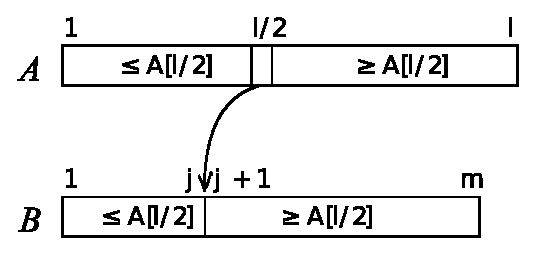
\includegraphics[width=4in]{lecture21/merge-sort.eps}
  \caption{Распараллеливание Merge}
  \label{fig:merge-sort}
\end{figure}

Для объединения двух массивов (они могут быть даже разной длины), берём больший
из них, находим его медиану (т.к. массив отсортирован -- это будет простым
вычислением индекса, константная операция). Затем с помощью бинарного поиска
ищем во втором (меньшем) массиве то место, на котором должна находиться
найденная медиана. После этого мы получим во втором массиве слева -- элементы
меньшие медианы, справа -- большие. Соответственно теперь задачу можно разделить
на две параллельные составляющие -- объединение левых частей массивов и правых.
А затем просто сконкатенировать результаты.

\begin{codebox}
\Procname{$\proc{P-Merge}(A[1 \twodots l], B[1 \twodots m], C[1 \twodots n]$}
\li \Comment объединяем $A$ и $B$ в $C$, длина $n = l + m$
\li \Comment не теряя общности предполагаем, что $l > m$
\li рассматриваем базовый случай 
\li ищем такое $j$, что $B[j] \leqslant A[l/2] \leqslant B[j+1]$ двоичным поиском
\li \textbf{spawn} $\proc{P-Merge}(A[1 \twodots (l/2)], B[1 \twodots j], C[1
  \twodots (l/2 + j)]))$
\li \textbf{spawn} $\proc{P-Merge}(A[(l/2+1) \twodots l], B[(j+1) \twodots m], C[(l/2+j+1)
  \twodots n])$
\li \textbf{sync}
\li \Return
\end{codebox}

\textbf{Анализ}:

Оценим в начале длину критического пути. Поскольку мы используем больший массив
для нахождения медианы, получается, что как минимум четверть элементов будет
находиться в меньшей из подзадач. Таким образом мы достигаем константного,
ограниченного снизу разделения на подзадачи, что позволяет нам сделать оценки.
Таким образом, размер большей подзадачи ограничен $3n/4$, что мы и используем в
рекуррентности. Бинарный поиск ограничен $\Theta(\lg n)$:

\begin{align*}
  PM_{\infty} &= PM_{\infty}(3n/4) + \Theta(\lg n) \\
    &= \Theta(\lg^2 n)
\end{align*}

Теперь оценим работу. Каждый раз задача разбивается на две подзадачи, пусть
коэффициент разбиения равен $\alpha$, тогда их размер равен $\alpha n$ и $(1 -
\alpha) n$, где $1/4 \leqslant \alpha \leqslant 3/4$. Тогда работа равна:

$$
PM_1 = PM_1(\alpha n) + PM_1((1 - \alpha)n) + \Theta(\lg n)
$$

Покажем, что работа $PM_1 = \Theta(n)$ с помощью метода подстановки.

Индуктивно предположим, что $PM_1(n) \leqslant an - b\lg n$ для неких констант
$a, b > 0$.

\begin{align*}
  PM_1(n) &\leqslant a\alpha n - b \lg (\alpha n) + \alpha (1 - \alpha) n - b
  \lg ((1 - \alpha) n) + \Theta(\lg n) \\
  &= an - b(\lg(\alpha n) + \lg ((1 - \alpha) n)) + \Theta(\lg n) \\
  &= an - b(\lg \alpha + \lg n + \lg(1- \alpha) + \lg n) + \Theta(n) \\
  &= an - b\lg n - (b(\lg n + \lg(\alpha(1 - \alpha))) - \Theta(\lg n)) \\
  &\leqslant an - b \lg n
\end{align*}

Так как мы можем выбрать $b$ достаточно большим для того, чтобы $b(\lg n +
\lg(\alpha(1 - \alpha)))$ доминировало надо $\Theta(\lg n)$. Также мы можем
выбрать $a$ достаточно большим, чтобы удовлетворить неравенство в базовом
случае. Таким образом, получили, что работа линейна, как и в случае с
непараллельным алгоритмом (однако константы, несомненно, больше).

Проведём анализ сортировки слиянием с использованием процедуры параллельного
слияния:

\begin{align*}
  M_{\infty}(n) &= M_{\infty}(n/2) + \Theta(\lg^2 n) = \Theta(\lg^3 n) \\
  \bar{P} &= \Theta(n \lg n / \lg^3 n) = \Theta(n / \lg^2 n)
\end{align*}

что значительно лучше предыдущего алгоритма.

Наилучшее же на сегодня решение обладает параллелизмом $\Theta(n / \lg n)$

\end{document}
